\documentclass[addpoints,11pt]{exam}

\usepackage{alltt}
\usepackage[margin=1in]{geometry}   % set up margins
\usepackage[T1]{fontenc}
\usepackage[usenames,dvipsnames]{xcolor}
\usepackage{enumerate}              % fancy enumerate
\usepackage{amsmath}                % used for \eqref{} in this document
\usepackage{amsthm}
\theoremstyle{definition}
\newtheorem{exmp}{Example}[section]
\usepackage{verbatim}               % useful for \begin{comment} and \end{comment}
\usepackage{eurosym}                % used for euro symbol
\usepackage{caption} 
\usepackage{graphicx}
\graphicspath{{Figures/}}
\usepackage{subcaption}
\usepackage{color}
\usepackage{float}
\usepackage{amssymb}
\usepackage{sgamevar}
\usepackage{sgame}
\usepackage[colorlinks=true]{hyperref}
\hypersetup{colorlinks=true, citecolor=ForestGreen, linkcolor=BlueViolet, urlcolor=Magenta}



%Solutions or nah (blank next two lines out for no solutions, unblank #3)
%\printanswers
%\newcommand{\dd}[1]{\par {\textbf{\textcolor{red}{#1}}}}
\newcommand{\dd}[1]{}  


\setlength\parindent{0pt}
\unframedsolutions
\SolutionEmphasis{\color{red}}
\CorrectChoiceEmphasis{\color{red}}
\renewcommand{\choicelabel}{(\alph{choice})}
\newcommand{\blank}[0]{\underline{\hspace{3cm}}}
\pointformat{\bfseries[\thepoints]}
\pointpoints{pt}{pts}
\pointsinrightmargin


\begin{document}


\title{\textbf{Homework 5} \\ \dd{Solutions \\} \vspace{2 mm} {\large ECON 101}}
\author{Summer I 2016}
\date{}
\maketitle

\makebox[\textwidth]{Name:\enspace\hrulefill}
\\

\makebox[\textwidth]{ONYEN:\enspace\hrulefill}
\\

\makebox[\textwidth]{PID:\enspace\hrulefill}
\\

\begin{center}
	\fbox{\fbox{\parbox{5.5in}{\centering
			This homework is due on \textbf{June 8} by \textbf{1PM}. Show work for all questions that require it (including multiple choice questions), attaching extra sheets as necessary. Multiple choice answers should be bubbled in on a scantron. For the short answer section, write legibly and make sure to box final answers. The total number of points available on this assignment is \textbf{100}.}}}
\end{center}

\subsection*{Multiple Choice [2 pts each]}

\begin{questions}
	

\question A closed economy has income of \$1,000, government spending of \$200, taxes of \$150, and investment of \$250. What is private saving?

\begin{choices}
	\choice \$100
	\choice \$200
	\CorrectChoice \$300
	\choice \$400
\end{choices}

\begin{solution}
	National saving = National investment. $Y - C - G = I$ $\Rightarrow 1000 - C - 200 = 250 \Rightarrow C = \$550$. Private saving = $Y - T - C = 1000 - 150 - 550 = \$300.$
\end{solution}

\question Acme, LLC is considering purchasing a new factory. If the interest rate falls, then the present value of the returns from the factory will \blank, and the company will be \\ \blank likely to build the factory.

\begin{choices}
	\choice increase; less
	\choice decrease; more
	\CorrectChoice increase; more
	\choice decrease; less
\end{choices}


\begin{solution}
	If the interest rate falls, then the cost of borrowing will decrease and so the present value of the returns increases. This will make the company more likely to build the factory.
\end{solution}


\newpage

\question If the business community becomes more optimistic about the profitability of capital, the \blank for loanable funds would shift, driving the equilibrium interest rate \\  \blank.

\begin{choices}
	\choice supply; up
	\choice supply; down
	\CorrectChoice demand; up
	\choice demand; down
\end{choices}

\begin{solution}
	Demand for loanable funds will increase, which will increase the equilibrium interest rate and quantity of loanable funds.
\end{solution}

\question Which of the following graphs of the loanable funds market correctly shows the effect of the imposition of a consumption tax?

\begin{figure}[ht]
	\begin{subfigure}[b]{0.5\textwidth}
		\centering
	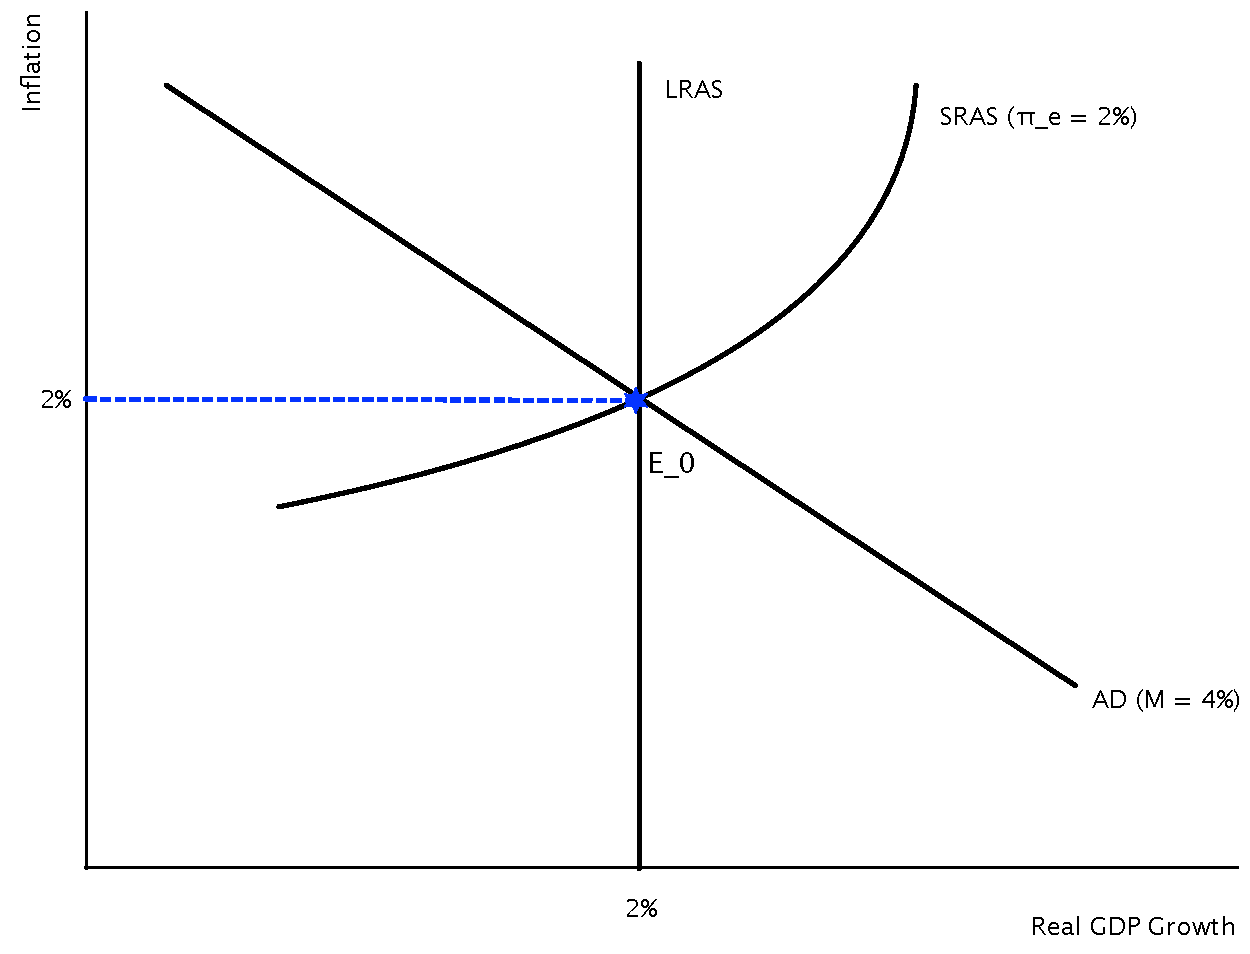
\includegraphics[scale=.35]{hw6_plot1.pdf}
		\caption{}
	\end{subfigure}
	\begin{subfigure}[b]{0.5\textwidth}
		\centering
	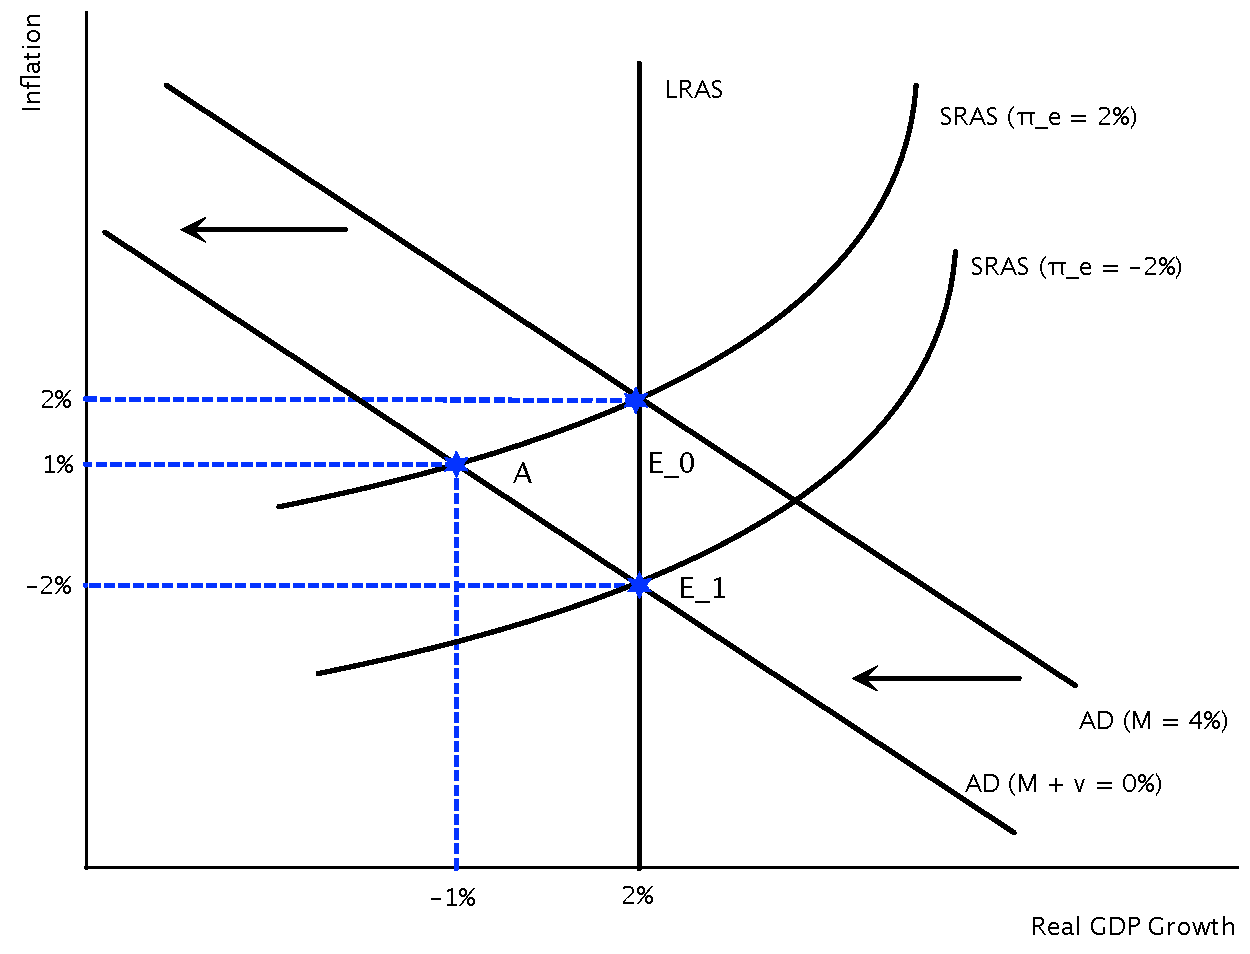
\includegraphics[scale=.35]{hw6_plot2.pdf}
		\caption{}
	\end{subfigure}
		%        
		
	\begin{subfigure}[b]{0.5\textwidth}
		\centering
		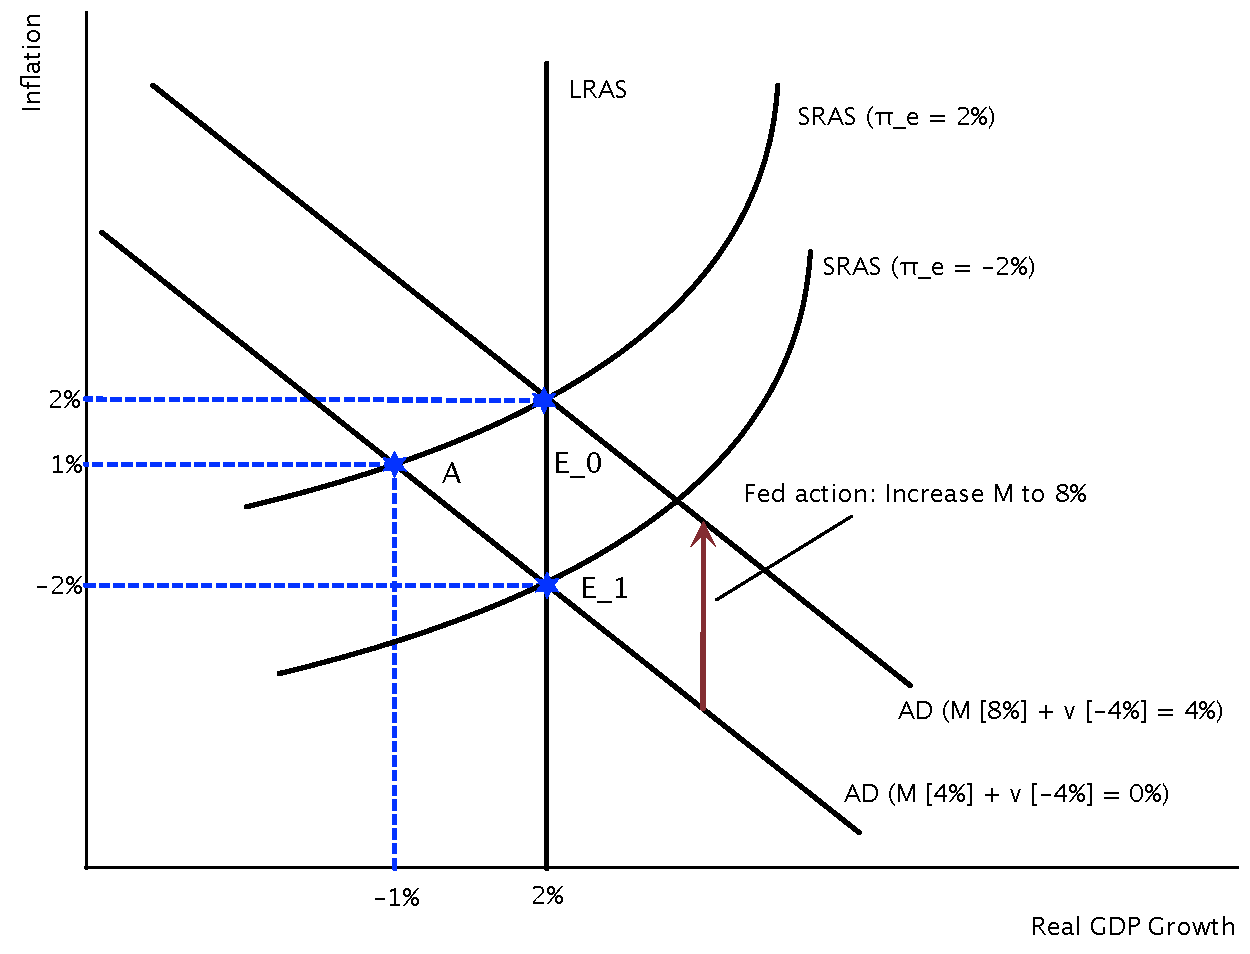
\includegraphics[scale=.35]{hw6_plot3.pdf}
		\caption{}
	\end{subfigure}
	\begin{subfigure}[b]{0.5\textwidth}
		\centering
		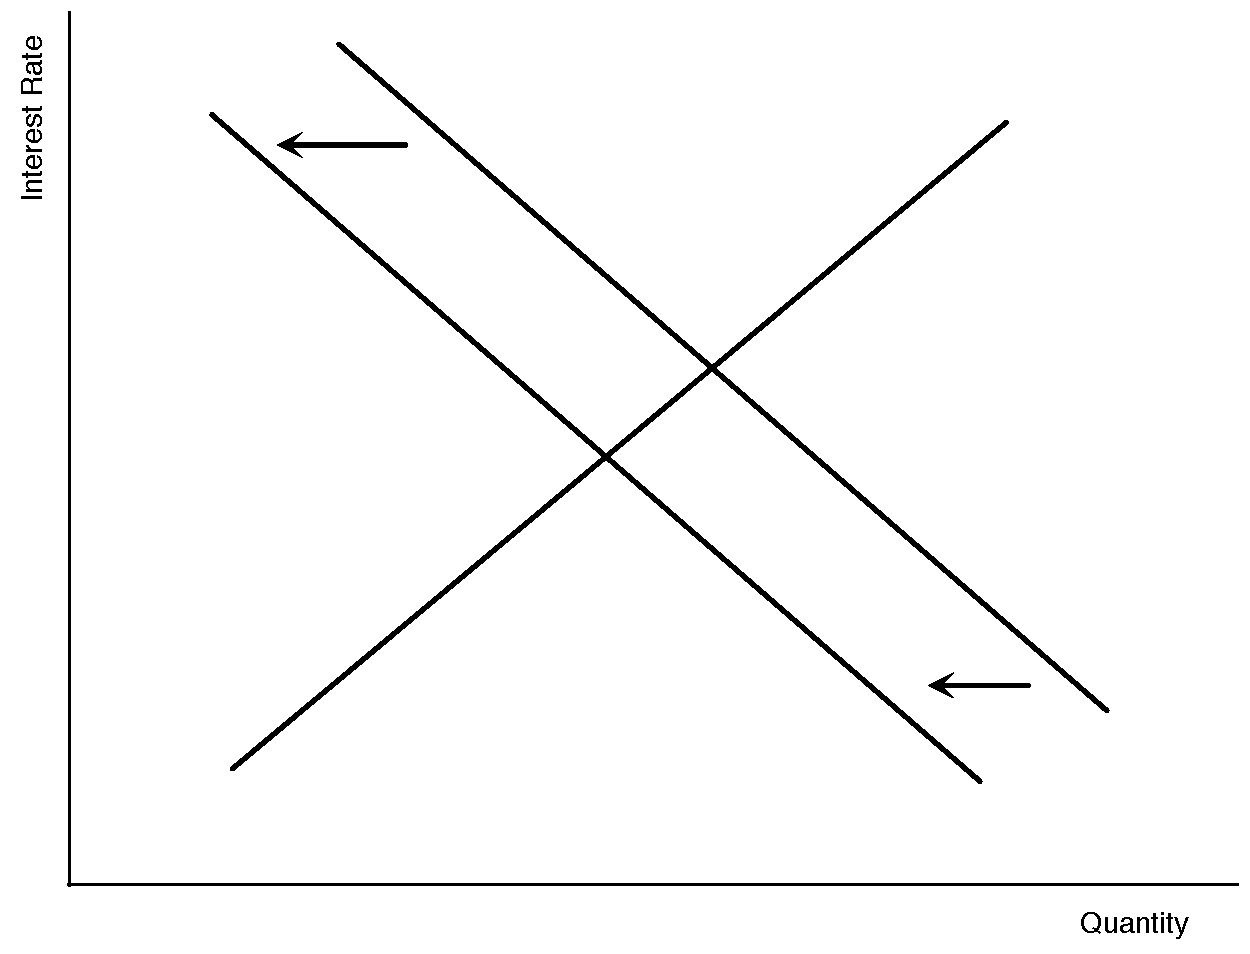
\includegraphics[scale=.35]{hw6_plot4.pdf}
		\caption{}
	\end{subfigure}
\end{figure}

\begin{solution}
	A tax on consumption provides an incentive for people to save more (since we assume you can either spend your income on savings or consumption) and so the supply of loanable funds will increase. Option (c) shows this shift.
\end{solution}

\question Always On Time Airlines is considering purchasing a new jet. The company would be \textit{less} likely to purchase a new jet if either

\begin{choices}
	\choice the price of a new jet decreased or the interest rate decreased.
	\choice the price of a new jet increased or the interest rate decreased.
	\choice the price of a new jet decreased or the interest rate increased.
	\CorrectChoice the price of a new jet increased or the interest rate increased.
\end{choices}

\begin{solution}
	The cost of borrowing increases if the price of the jet increases or interest rates increase.
\end{solution}

\newpage

\question What effect will an investment tax credit have on interest rates and the quantity of savings?

\begin{choices}
	\choice Both interest rates and the quantity of savings will decrease.
	\choice Interest rates will increase, and the quantity of savings will decrease.
	\CorrectChoice Both interest rates and the quantity of saving will increase.
	\choice Interest rates will decrease, and the quantity of savings will increase.
\end{choices}

\begin{solution}
	An investment tax credit will increase the demand for loanable funds. This will increase both the equilibrium interest rate and quantity of loanable funds.
\end{solution}
	
	\question Suppose you currently hold a bond that promises to pay \$100 in a year, \$100 in two years, and \$1,100 in three years. If you wish to sell the bond today in order to buy a new bicycle, which of the following market interest rates would allow you to sell the bond for the highest price?
	
	\begin{choices}
		\choice 7\%
		\choice 10\%
		\CorrectChoice 5\%
		\choice 8\%
	\end{choices}
	
\begin{solution}
	The price of a bond is inversely related to market interest rates.
\end{solution}

\question Assuming the supply of loanable funds is made up of national savings, which of the following would be the most likely to cause an increase in the demand for loanable funds?

\begin{choices}
	\choice A decrease in the interest rate.
	\choice An increase in savings.
	\choice A decrease in consumption.
	\choice An increase in government borrowing.
	\CorrectChoice None of the above.
\end{choices}

\begin{solution}
	(b) - (d) all affect the supply of loanable funds, while (a) causes a movement along the curves.
\end{solution}
	
	\question Other things the same, an increase in the minimum wage 
	
	\begin{choices}
		\choice increases frictional unemployment but leaves the natural rate of unemployment unchanged.
		\choice  increases frictional unemployment and increases the natural rate of unemployment.
		\choice  increases structural unemployment but leaves the natural rate of unemployment unchanged.
		\CorrectChoice increases structural unemployment and increases the natural rate of unemployment.
	\end{choices}
	
	\begin{solution}
		The minimum wage would increase structural unemployment, which in turn would increase the natural rate of unemployment.
	\end{solution}
	
	\question If an unemployed person quits looking for work, then eventually the unemployment rate will \blank and the labor force participation rate will \blank.
	
	\begin{choices}
		\choice decrease; remain the same
		\CorrectChoice decrease; decrease
		\choice remain the same; decrease
		\choice remain the same; remain the same
	\end{choices}
	
	\begin{solution}
		The discouraged worker would no longer be counted as unemployed or as in the labor force, so both the unemployment rate and LFPR would decrease.
	\end{solution}
	
		\question The actual unemployment rate varies around the 
		
		\begin{choices}
			\choice frictional unemployment rate.
			\choice structural unemployment rate.
			\choice cyclical unemployment rate. 
			\CorrectChoice natural unemployment rate.
		\end{choices}
		
		\begin{solution}
			See class notes.
		\end{solution}
		
	\newpage
	
		\question Natalie just graduated from college. In order to devote all her efforts towards her education, she didn't hold a job while in school. Now, she is going to cruise around the country on her motorcycle for awhile before she starts looking for work. As a result, the unemployment rate
		
		
		\begin{choices}
			\choice increases, and the labor-force participation rate increases.
			\CorrectChoice is unaffected, and the labor-force participation rate is unaffected.
			\choice increases, and the labor-force participation rate decreases. 
			\choice increases, and the labor-force participation rate is unaffected.
		\end{choices}
		
		\begin{solution}
			Natalie was not in the labor force as a student, and will still not be in the labor force while she is not looking for a job. Thus, neither the unemployment rate or LFPR are affected.
		\end{solution}
	
	\question John Doe looked for a new job for two months when he and his family moved to South Florida, but stopped looking for work six weeks ago because his wife landed a prominent position at the University of Miami. As of right now, John is considered \underline{\hspace{3cm}} by the BLS.
	\begin{choices}
		\choice frictionally unemployed.
		\choice structurally unemployed. 
		\choice cyclically unemployed.
		\CorrectChoice not in the labor force.
	\end{choices}

	\begin{solution}
		John has not actively sought work in the last 4 weeks, so he would not be included in the labor force.
	\end{solution}

	\question Consider Table \ref{MC28}, which shows the people in country $Y$ that are structurally unemployed, cyclically unemployed, and frictionally unemployed. 
	
	
	\begin{table}[H]
		\caption{Unemployment Statistics for Country $Y$}
		\centering
		\begin{tabular}{  c | c} 
			
			Type of Unemployment & Number Unemployed\\
			\hline
			Structural &  14 million\\
			Cyclical &  8 million\\
			Frictional & 10 million\\
		\end{tabular}
		\label{MC28}
	\end{table}
	
	
	
	Additionally, there are 300 million people employed and 350 million adults in the country. What is the natural unemployment rate?
	
	\begin{choices}
		\CorrectChoice 7.2\%
		\choice 8.0\%
		\choice 9.1\%
		\choice 9.6\%
	\end{choices}
	
	\begin{solution}
		Natural unemployment rate = (structural + frictional unemployment)/(Labor force) = (14 + 10)/(300+14+8+10) = 7.2\%.
	\end{solution}
	
	\question Suppose an economy has 139.2 million adults that are employed, 14.5 million that are unemployed, and 85.2 million that are not in the work force. Given this information, what is the unemployment rate?
	
	\begin{choices}
		\choice 6.1\%
		\CorrectChoice 9.4\%
		\choice 10.4\%
		\choice 8.7\%
	\end{choices}
	
	\begin{solution}
		Unemployment rate = \#unemployed/labor force = 14.5/(139.2+14.5) = 9.4\%.
	\end{solution}
	
	\newpage
	
	\question Frictional unemployment is best defined as 
	
	\begin{choices}
		\choice long-term unemployment caused by changing features of an economy.
		\CorrectChoice short-term unemployment caused by difficulties of matching employees to employers.
		\choice unemployment caused by cyclical conditions of an economy.
		\choice a normal level of unemployment caused by high wages. 
	\end{choices}
	
	
	\question While cleaning your apartment, you look under the sofa cushion and find a \$50 bill. You deposit the bill in your checking account. The Fed's reserve requirement is 20\% of deposits. What is the maximum amount that the money supply could increase?
	
	\begin{choices}
		\choice \$10
		\choice \$50
		\CorrectChoice \$200
		\choice \$250
	\end{choices}
	
	\begin{solution}
		Your deposit will could increase the money supply through the banking system by $50 \times 1/.20 = \$250$, but you removed \$50 in currency and so the maximum increase in the MS is \$200.
	\end{solution}
	
	
	\question Chloe takes \$100 of currency from her wallet and deposits it in a checking account. If the bank adds the entire \$100 to reserves, the money supply \blank, but if the bank lends out some of the \$100, the money supply \blank.
	
	\begin{choices}
		\choice increases; increases even more
		\choice increases; increases by less
		\CorrectChoice is unchanged; increases
		\choice decreases; decreases by less
	\end{choices}


	
	\question In a system of fractional-reserve banking, even without any action by the central bank, the money supply declines if households choose to hold \blank currency or if banks choose to hold \blank excess reserves.
	
	\begin{choices}
		\CorrectChoice more; more
		\choice more; less
		\choice less; more
		\choice less; less
	\end{choices}
	
	\begin{solution}
		If people hold more in currency, banks cannot lend out as much money. If banks hold excess reserves, they are not loaning as much money as they could be.
	\end{solution}

	\question Suppose an economy contains 2,000 \$1 bills. If people initially deposit half their currency as demand deposits while banks maintain 100\% reserves, the maximum quantity of money would be \blank. If, however, people initially deposit half their currency as demand deposits while banks maintain 10\% reserves, the maximum quantity of money is \blank.
	
	\begin{choices}
		\choice \$2,000; \$10,000
		\choice \$1,000; \$10,000
		\choice \$1,000; \$11,000
		\CorrectChoice \$2,000; \$11,000
	\end{choices}

	\begin{solution}
		In a 100\% reserve banking system, the money supply does not change if people hold money in deposits. \$1,000 are in currency, \$1,000 are in deposits. Under a fractional-reserve system, money is created. \$1,000 are in currency, and \$1,000 $\times$ 1/.10 = \$10,000 are potentially created by the banking system.
	\end{solution}
	
\newpage

\question If the Fed wanted to increase the money supply, it could

\begin{choices}
	\CorrectChoice purchase government bonds.
	\choice increase the required reserve ratio.
	\choice increase the discount rate.
	\choice increase the interest rate on reserves.
\end{choices}


\question Suppose a shift in the money supply caused the value of money to decrease from $1/4$ to $1/5$. As such, the price level in the economy

\begin{choices}
	\choice decreased 20\%.
	\CorrectChoice increased 25\%.
	\choice increased 20\%.
	\choice decreased 25\%.
\end{choices}

\begin{solution}
	Value of money = 1/P $\Rightarrow P_0 = 4$, $P_1 = 5$. $\%\Delta P = (5-4)/4 \times 100\% = +25\%$.
\end{solution}

\question Suppose the interest rate on a home mortgage was set with the expectation that the price level would decrease by 3\%. If through the course of the loan, the price level actually did not change, who was hurt most?

\begin{choices}
	\choice The mortgage holder
	\CorrectChoice The bank
	\choice Neither was hurt
	\choice Both were hurt equally
\end{choices}

\begin{solution}
	Actual inflation was greater than expected inflation, so lenders are hurt.
\end{solution}

\question You put money in an account that advertises a 5\% interest rate. The inflation rate is 3\%, and the tax rate on your returns is 20\%. Your after-tax nominal rate of interest is \blank and your after-tax real rate of interest is \blank.

\begin{choices}
	\choice 1\%; 2\%
	\choice 1\%; .8\%
	\CorrectChoice 4\%; 1\%
	\choice 4\%; .8\%
\end{choices}

\begin{solution}
	After-tax nominal rate = 5\% $\times$ (1-.20) = 4\%. After-tax real rate = 4\% - 3\% = 1\%.
\end{solution}

\question An economy produces one good -- rice. The economy has enough labor, capital, and land to produce 800 bags. The money supply in this economy is \$2,000 and rice sells for \$5/bag. The nominal GDP in the economy is \blank and the velocity of money is \blank.

\begin{choices}
	\CorrectChoice \$4,000; 2
	\choice \$2,000; 2
	\choice \$4,000; 1
	\choice \$2,000; 1
\end{choices}

\begin{solution}
	Quantity Theory of Money (in levels): $Mv=PY$, where $PY$ = \$5 $\times$ 800 = \$4,000 = nominal GDP. $v$ = 4000/2000 = 2.
\end{solution}

\newpage

\question According to the quantity theory of money and the Fisher effect, if the central bank increases the rate of money growth

\begin{choices}
	\CorrectChoice inflation and the nominal rate will both increase. 
	\choice inflation and the real interest rate both increase.
	\choice the nominal interest rate and the real interest rate both increase.
	\choice inflation, the real interest rate, and the nominal interest rate all increase.
\end{choices}


\question According to the quantity theory of money, an increase in the money supply will cause the price level to 

\begin{choices}
	\choice remain relatively constant since money is neutral.
	\CorrectChoice increase by the same percentage as the money supply.
	\choice increase by a greater percentage than the money supply.
	\choice increase by a smaller percentage than the money supply.
\end{choices}


\question Consider Figure \ref{MC8}, which shows the market for money in Portlandia. $P$ is the overall price level in the economy.

\begin{figure}[H]
	\centering
	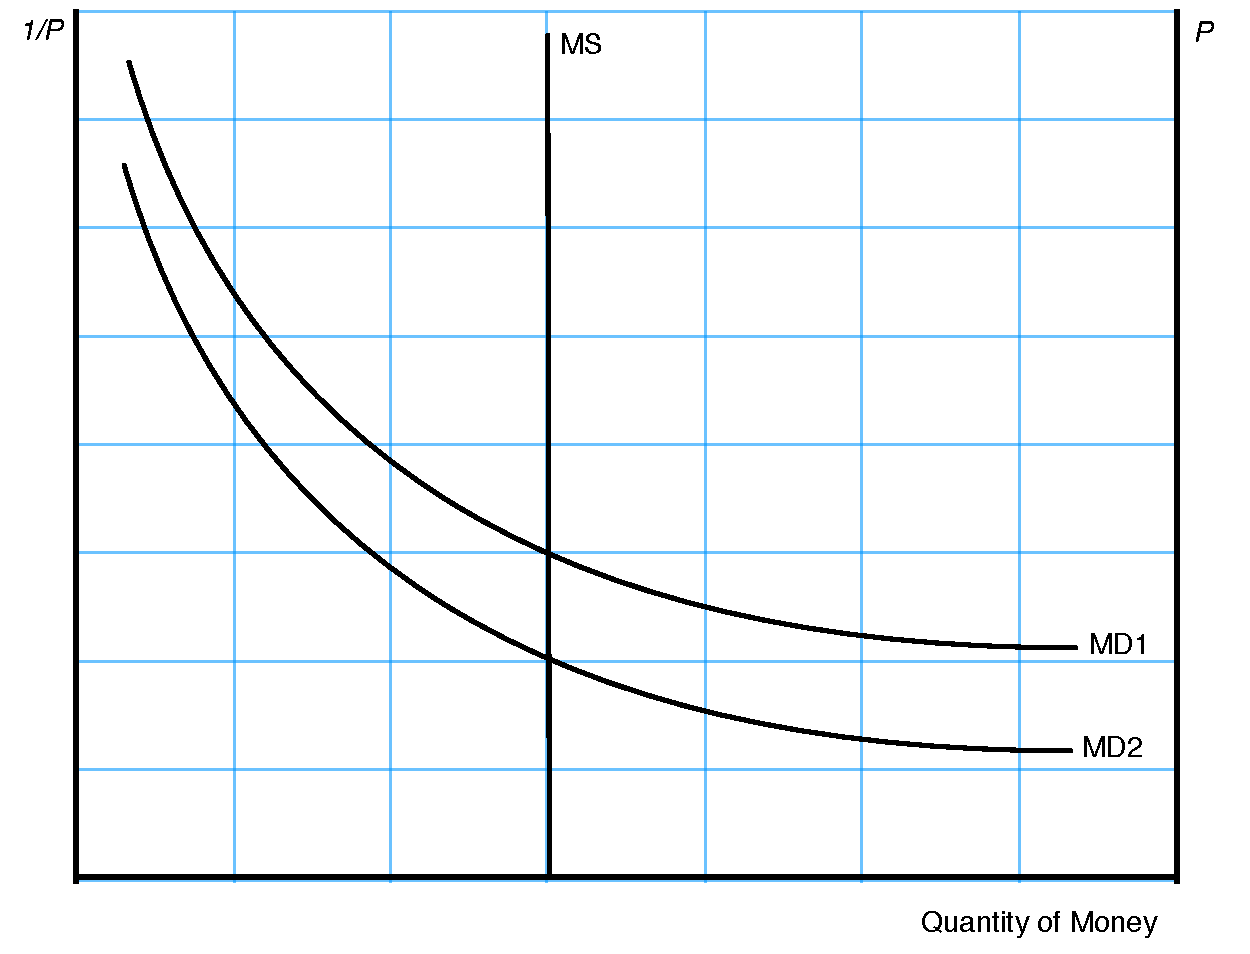
\includegraphics[scale=.40]{Final_MC8.pdf}
	\caption{The Money Market}
	\label{MC8}
\end{figure}

If the demand for money shifts from MD1 to MD2, then we can say that 

\begin{choices}
	\choice the value of money will increase, while the price level will decrease.
	\choice the value of money and the price level will both increase.
	\CorrectChoice the value of money will decrease, while the price level will increase.
	\choice the value of money and the price level will both decrease.
\end{choices}

\begin{solution}
	A decrease in money demand will decrease the value of money and increase the price level (y-axis on the right is inverted).
\end{solution}

\newpage

\question Which of the following is NOT a cost of inflation?

\begin{choices}
	\choice Shoeleather costs
	\CorrectChoice Relative-price stability
	\choice Arbitrary redistribution of wealth
	\choice Menu costs
\end{choices}


\question Unexpected deflation will

\begin{choices}
	\choice lower the real value of debts and redistribute wealth from lenders to borrowers.
	\choice lower the real value of debts and redistribute wealth from borrowers to lenders.
	\choice raise the real value of debts and redistribute wealth from lenders to borrowers.
	\CorrectChoice raise the real value of debts and redistribute wealth from borrowers to lenders.
\end{choices}

\begin{solution}
	Unexpected deflation implies that actual inflation is less than expected, which increases the real value of debts and so wealth is transferred from borrowers to lenders.
\end{solution}
		
\end{questions}


\subsection*{Short Answer}

\begin{questions}


	\question Three students have each saved \$500. Each has an investment opportunity in which he or she can invest up to \$1,000. The rates of return on the investment projects are as follows:
	
		
		\begin{table}[H]
			\caption{Rates of Return}
			\label{tab1}
			\centering
			\begin{tabular}{  c|c}        
				
				Student   & Rate of Return ($r$) \\
				\hline
				Natalie & 5\% \\
				Isabella & 8\% \\
				Noah & 15\% \\
			\end{tabular}
		\end{table}
	
	\begin{parts}
		\part[2] Suppose their school opens a market for loanable funds in which students can lend and borrow among themselves at interest rate $i$. What would determine whether a student would choose to be a borrower or a lender in this market? 
		
		\begin{solution}
			If $i>r$, the student would rather lend since they would get a higher return on a loan than on their investment. If $i<r$, the student would rather borrow.
		\end{solution}
		\part[4] Among these three students, what would be the quantity of loanable funds supplied and quantity demanded at an interest rate of 7\%? At 10\%? 
		
		\begin{solution}
			At $i=7\%$, Natalie would be a lender while Isabella and Noah would be borrowers. $Q_s$ = \$500, $Q_d$ = \$1,000. At $i=10\%$, Natalie and Isabella would be lenders while Noah would a be borrower. $Q_s$ = \$1,000, $Q_d$ = \$500.
		\end{solution}
		
		\part[4] At what interest rate would the loanable funds market among these students be in equilibrium? Which student(s) would be borrowers and which would be lenders? 
		
		\begin{solution}
			$i^* = 8\%$. Natalie would lend \$500 ($Q_s$), Noah would borrow \$500 ($Q_d$, and Isabella uses her own funds to invest and would neither borrow or lend.
		\end{solution}
		
		\part[4] At this equilibrium interest rate, how much does each student have a year later after the investment projects pay their returns and loans have been repaid? 
		
		\begin{solution}
			Isabella invests \$500 and gets an 8\% return: \$500(1.08) = \$540.\\
			Natalie lends \$500 and gets 8\% interest: \$500(1.08) = \$540.\\
			Noah borrows \$500 at 8\% and invests \$1,000 with a 15\% return: \$1,000(1.15) - \$500(1.08) = \$610.
		\end{solution}
	
	\end{parts}
		
		\question Suppose an economy contains 5,000 \$1 bills.
		\begin{parts}
			\part[2] If people initially deposit all their currency as demand deposits and banks maintain 100\% reserves, what is the maximum quantity of money? 
			\begin{solution}
				\$5,000, all in deposits.
			\end{solution}
			\part[2] If people initially deposit half their currency as demand deposits and banks maintain 100\% reserves, what is the maximum quantity of money? 
			\begin{solution}
				\$5,000. \$2,500 in currency, \$2,500 in deposits.
			\end{solution}
			\part[2] If people initially deposit half their currency as demand deposits and banks maintain 10\% reserves, what is the maximum quantity of money? 
			\begin{solution}
				\$27,500. \$2,500 $\times$ 1/.10 = \$25,000 in deposits, \$2,500 in currency.
			\end{solution}
			\part[4] Banks always maintain the minimum required reserve ratio set by the central bank (i.e., they hold no excess reserves). If the central bank decreased this requirement to 5\%, what would be the effect on the money supply? What if it increased the requirement to 15\%? 
			\begin{solution}
				Decreasing the reserve requirement would increase the quantity of money to \$2,500 + \$2,500 $\times$ 1/.05 = \$52,500. Increasing the reserve requirement would decrease the quantity of money to \$2,500 + \$2,500 $\times$ 1/.15 = \$19,166.67.
			\end{solution}
		\end{parts}
		
\newpage
		
		\question Suppose that this year's money supply is \$500 billion, nominal GDP is \$10 trillion, and the real GDP is \$5 trillion. 
		
		\begin{parts}
			\part[4] What is the price level? What is the velocity of money? 
			\begin{solution}
				$Mv=PY$, where $PY$ = nominal GDP. $P$ = nominal GDP/real GDP = 10,000/5,000 = 2. Velocity = $PY/M$ = 10,000/500 = 20.
			\end{solution}
			\part[4] Suppose that velocity is constant and the economy's output of goods and services rises by 5\% each year. What will happen to nominal GDP and the price level next year if the Fed keeps the money supply constant?
			\begin{solution}
				$\vec{M} + \vec{v} = \vec{Y} + \pi$. $\vec{v} = 0$, $\vec{Y} = 5\%$. If $\vec{M} = 0$, 0\% + 0\% = 5\% + $\pi \Rightarrow \pi = -5\%$. Prices will decrease by 5\% and nominal GDP will be unchanged.
			\end{solution}
			\part[4] What money supply should the Fed set next year if it wants to keep the price level stable? 
			\begin{solution}
				$\pi^* = 0\% \Rightarrow \vec{M}^* + 0\% = 5\% + 0\% \Rightarrow \vec{M}^* = 5\%$. $MS_1 = 500(1.05) = 525$B.
			\end{solution}
			\part[4] What money supply should the Fed set next year if it wants an inflation of 10\%?
			\begin{solution}
				$\pi^* = 10\% \Rightarrow \vec{M}^* + 0\% = 5\% + 10\% \Rightarrow \vec{M}^* = 15\%$. $MS_1 = 500(1.15) = 575$B.
			\end{solution}
		\end{parts}
	
	\question What topics or questions gave you the most trouble on this homework assignment or the class material it encompassed? 
\end{questions}



\end{document}

